\newcommand{\trans}[1]{[\![\texttt{#1}]\!]}
\newcommand{\atrans}[1]{\trans{#1}^\sharp}
\lstset{basicstyle=\small}
\newcommand{\example}[3]{
\input{#1/examples/example#2.tex}
\begin{figure}[h!]
\centering
\begin{subfigure}{.5\textwidth}
  \centering
  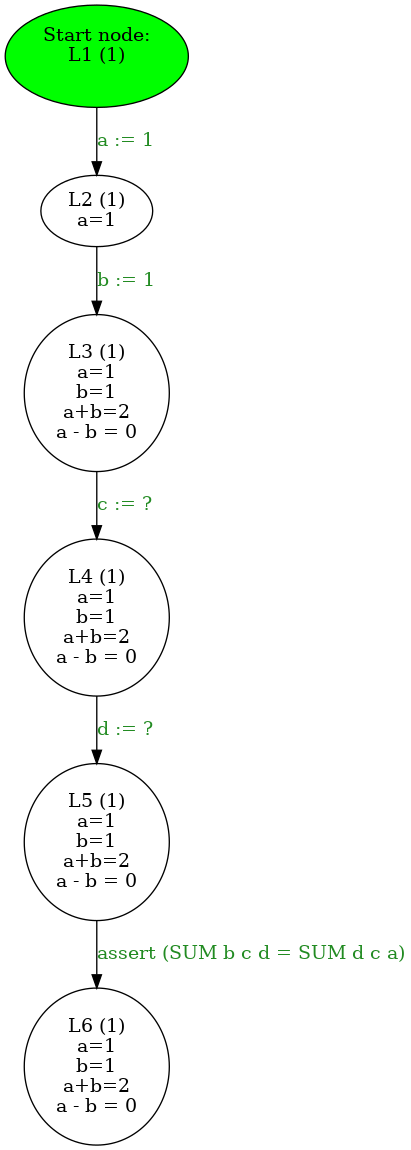
\includegraphics[height=#3\textheight]{./#1/examples/example#2-output/cfg.png}
  \caption{Control flow graph}
\end{subfigure}%
\begin{subfigure}{.5\textwidth}
  \centering
  \lstset{basicstyle=\small}
  \lstinputlisting{#1/examples/example#2.code}
  \caption{Code}
\end{subfigure}
\caption*{\texttt{pipenv run analyze --type #1 docs/#1/examples/example#2.code}}
\end{figure}
}

\newcommand{\parfBasis}[1]{(#1_{even}\leftrightarrow\neg #1_{odd})}